\documentclass[11pt]{article}
\usepackage[utf8]{inputenc}	% Para caracteres en español
\usepackage{amsmath,amsthm,amsfonts,amssymb,amscd}
\usepackage{multirow,booktabs}
\usepackage[table]{xcolor}
\usepackage{fullpage}
\usepackage{lastpage}
\usepackage{enumitem}
\usepackage{fancyhdr}
\usepackage{mathrsfs}
\usepackage{wrapfig}
\usepackage{setspace}
\usepackage{calc}
\usepackage{multicol}
\usepackage{cancel}
\usepackage[retainorgcmds]{IEEEtrantools}
\usepackage[margin=1cm]{geometry}
\usepackage{amsmath}
\newlength{\tabcont}
\setlength{\parindent}{0.0in}
\setlength{\parskip}{0.05in}
\usepackage{empheq}
\usepackage{framed}
\usepackage[most]{tcolorbox}
\usepackage{xcolor}
\usepackage{graphicx}
\usepackage{listings}
% -- Basic formatting
\usepackage[utf8]{inputenc}
\usepackage[english]{babel}
\usepackage{times}
\usepackage{caption}
\usepackage{subcaption}
\usepackage{placeins}
\setlength{\parindent}{0pt}
\usepackage{indentfirst}% -- Defining colors:
\usepackage[dvipsnames]{xcolor}
\definecolor{codegreen}{rgb}{0,0.6,0}
\definecolor{codegray}{rgb}{0.5,0.5,0.5}
\definecolor{codepurple}{rgb}{0.58,0,0.82}
\definecolor{backcolour}{rgb}{0.95,0.95,0.92}% Definig a custom style:
\lstdefinestyle{mystyle}{
    backgroundcolor=\color{backcolour},   
    commentstyle=\color{codepurple},
    keywordstyle=\color{NavyBlue},
    numberstyle=\tiny\color{codegray},
    stringstyle=\color{codepurple},
    basicstyle=\ttfamily\footnotesize\bfseries,
    breakatwhitespace=false,         
    breaklines=true,                 
    captionpos=t,                    
    keepspaces=true,                 
    numbers=left,                    
    numbersep=5pt,                  
    showspaces=false,                
    showstringspaces=false,
    showtabs=false,                  
    tabsize=2
}% -- Setting up the custom style:
\lstset{style=mystyle}
\lstset{
  style=mystyle,
  framexleftmargin=3.5mm,
  rulesepcolor=\color{black},
  linewidth=0.6\linewidth,
  xleftmargin=12pt,
  aboveskip=12pt,
  belowskip=12pt
}
\colorlet{shadecolor}{orange!15}
\parindent 0in
\parskip 1pt
\geometry{margin=1in, headsep=0.25in}
\theoremstyle{definition}
\newtheorem{defn}{Definition}
\newtheorem{reg}{Rule}
\newtheorem{exer}{Exercise}
\newtheorem{note}{Note}
\graphicspath{ {./images/} }
\begin{document}
\setcounter{section}{0}
\title{MIE223 Lecture Notes}

\thispagestyle{empty}

\begin{center}
{\LARGE \bf Feature Analysis and Visualization}\\
{\large MIE223}\\
Winter 2025
\end{center}
\section{Feature Analysis and Visualization}
\subsection{Exploratory Data Analysis (EDA)}
John Tukey (Bell Labs, 1970’s) (Inventor of the box-plot)
\begin{itemize}
  \item The first time corporations had a lot of digital data
  \item Data on semiconductor processes, networks
\end{itemize}

Observed that statistics was preoccupied with
hypothesis testing
\begin{itemize}
  \item But there were no established methodologies for
  \textbf{generating (data-driven) hypotheses}
  \item Espoused a visual methodology and a new language
  S (R became the free version)
\end{itemize}
\subsection{Data Science Process}
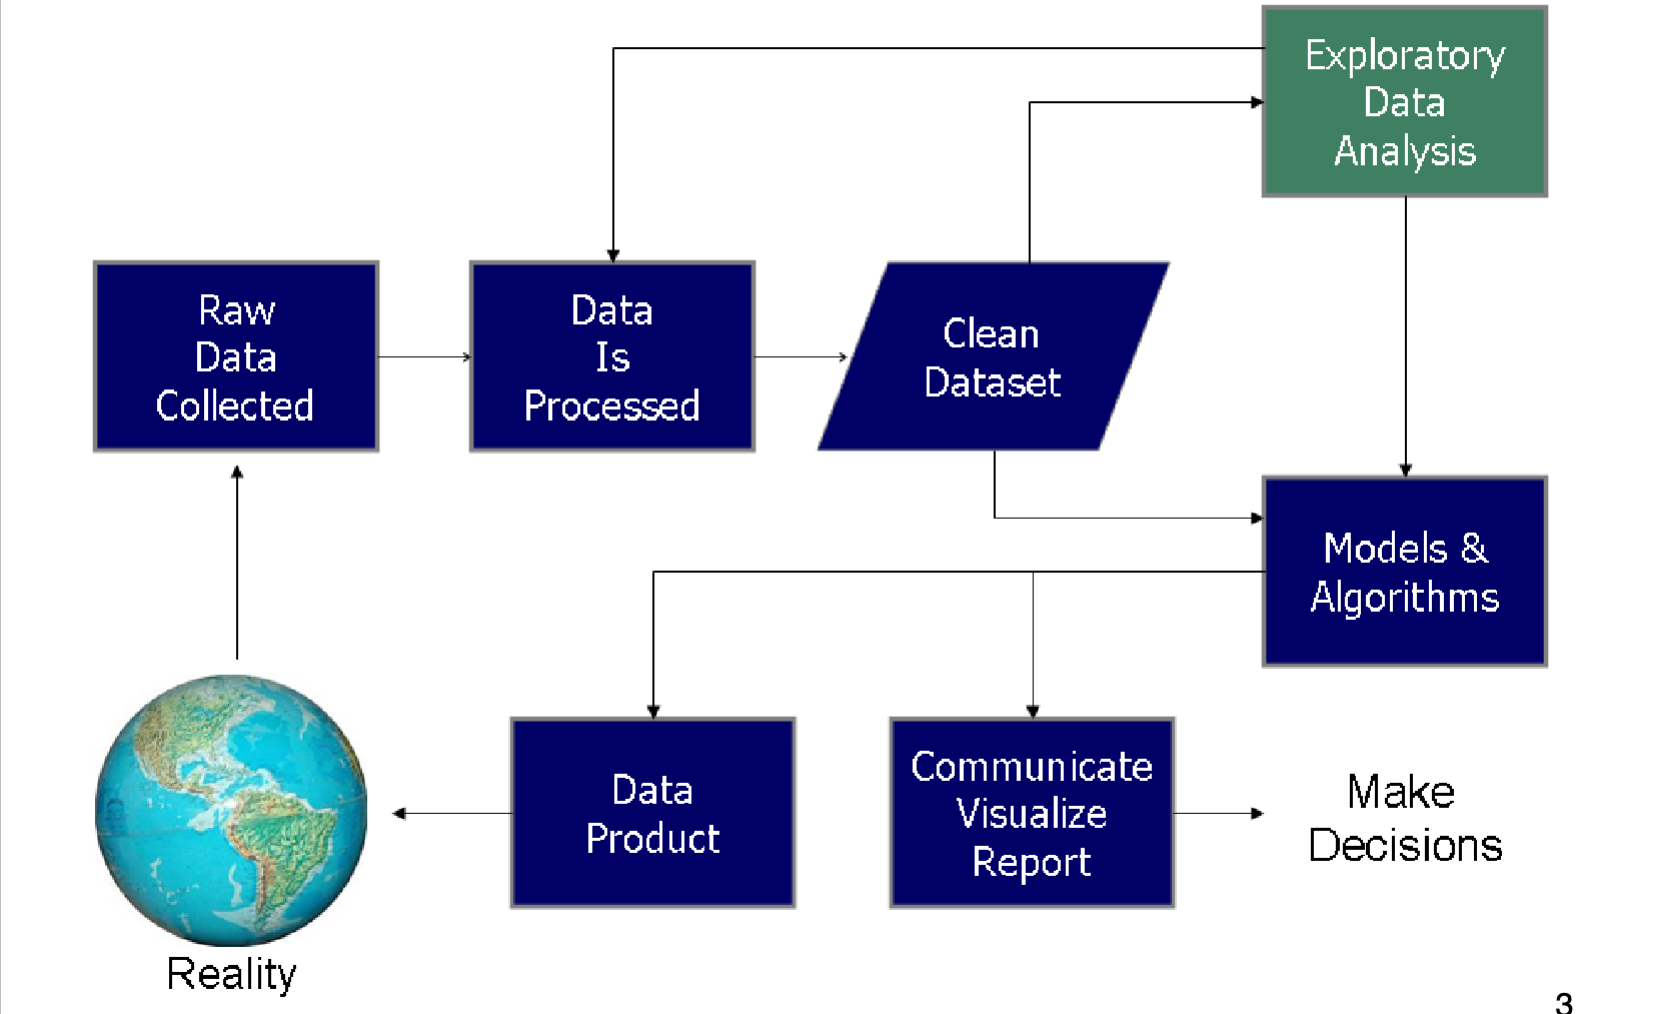
\includegraphics[width=\textwidth]{1.png}

\subsection{Data Cleaning: Brief Recap}
~80\% of your Data Science time

Some pointers:
\begin{itemize}
  \item Missing values – do not
  replace with 0 or -999
  \item Treat as missing
  \item Look for frequencies of
  values or outliers (-999)
  \begin{itemize}
    \item \textbf{Histograms} invaluable
    \item Examine \textbf{outliers} 
  \end{itemize}
  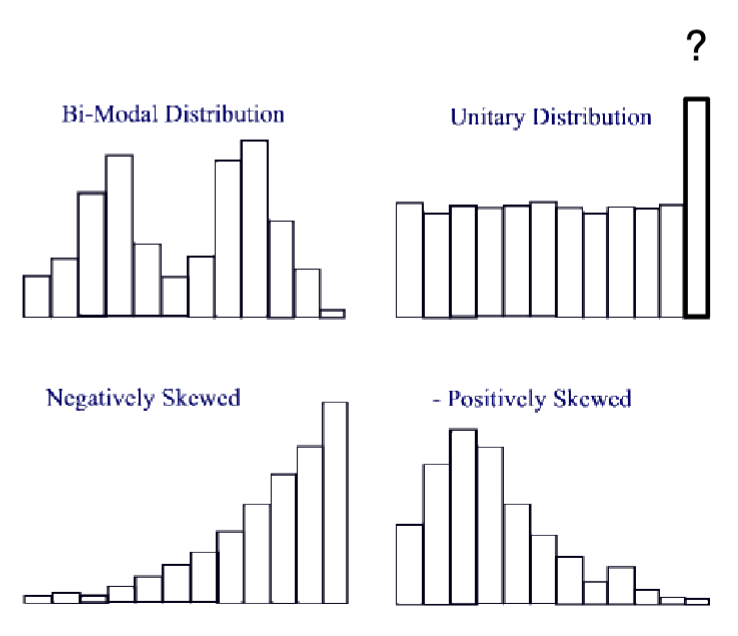
\includegraphics[width=\textwidth-27.37506pt]{2.png}
\end{itemize}
\section{Correlation}
We’ll be look at feature distributions
independently (per column), but also
relationships between features (columns).
Correlation is one of the first tools you think of
for looking at the relationship between two
features (but has limitations)
\subsection{Correlated variables}
Two variables are correlated if changes in one
variable, correspond to changes in the other

Correlation in general refers to the statistical
association between two variables
\begin{itemize}
  \item This statistical association allows us to make
  estimates for the one variable based on the value of
  the other
  \item While we typically think of linear relationships
  between variables, nonlinear might exist too
\end{itemize}
\subsection{Linear correlation}
\begin{itemize}
  \item Two variables x and y are said to be
  linearly correlated if their relationship can
  be described by the following equation:
\end{itemize}
\begin{equation}
  y = \alpha + \beta x, \beta \neq 0
\end{equation}
\begin{itemize}
  \item This relationship will not be exact
  \item There will be an error associated with it, and
  hence, in reality:
  \item $\epsilon$ is the error term for the relationship
\end{itemize}
\begin{equation}
  y = \alpha + \beta x + \epsilon, \beta \neq 0
\end{equation}
\subsection{Pearson correlation coefficient}
\begin{itemize}
  \item In order to test the linear association
  between two variables x and y we can use
  the Pearson correlation coefficient r$_{xy}$

  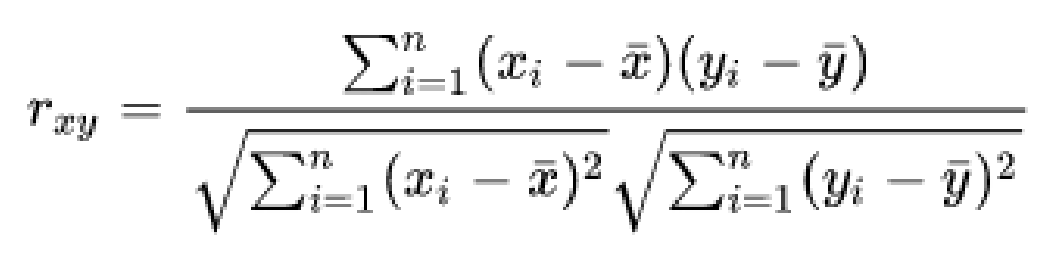
\includegraphics[width=\textwidth/2]{3.png}
  \item Pearson correlation is in the range [-1,1]
  \begin{itemize}
    \item 1: perfect/strong and positive linear correlation
    \item -1: perfect/strong and negative linear correlation
    \item 0: no linear correlation
  \end{itemize}
  \item It is very crucial to understand that this
  correlation coefficient can only examine
  linear associations between two variables

  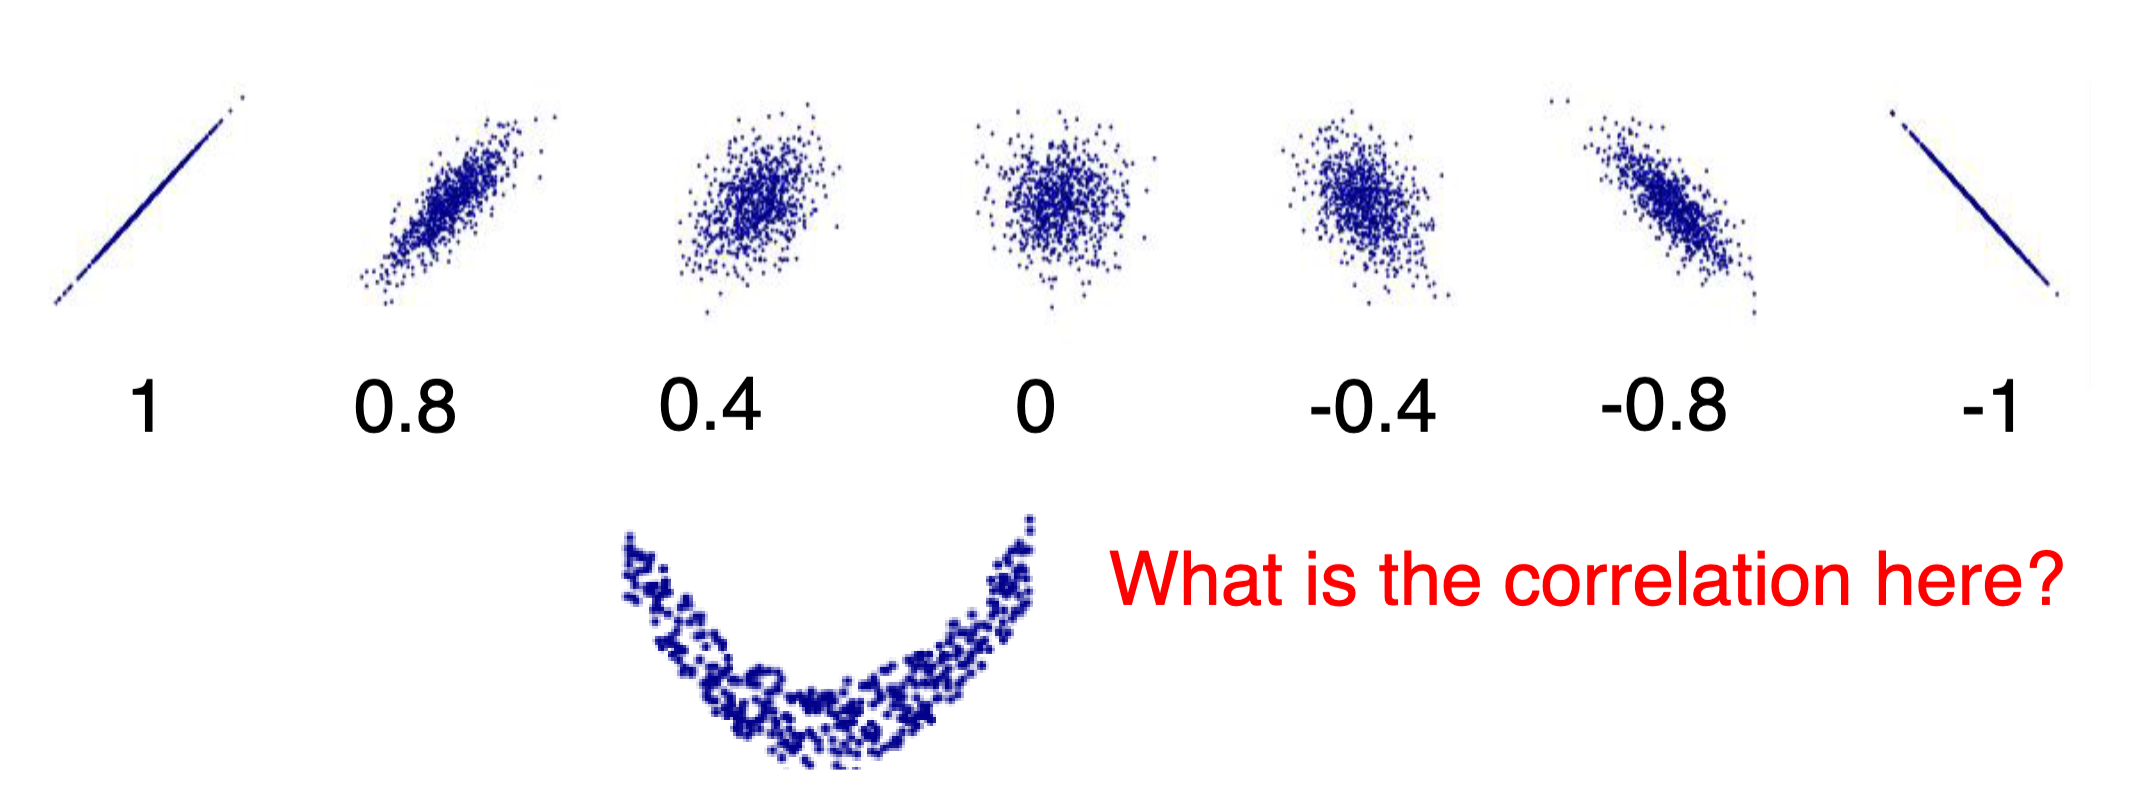
\includegraphics[width=\textwidth/2]{4.png}
\end{itemize}
\begin{note}
  \begin{itemize}
    \item Pearson correlation coefficient is sensitive to
    outliers
    \item It is not robust to outliers
    \item It is not a good measure of correlation for
    non-linear relationships
  \end{itemize}
\end{note}
\section{Feature Analysis: Probability Recap}
This is mathematical so we first
we need to make sure everyone
has the same understanding and
intuition for notation
\subsection{Random Variables}
\begin{itemize}
  \item Random variable (RV) denoted by uppercase letter (e.g. X)
  \item RVs take value assignments X = x where X is a
  \begin{itemize}
    \item Discrete RV if x is in a countable set (binary: x $\in$ {0,1}; or dice)
    \item Continuous RV if x is in an uncountable set (real: x $\in$ Reals)
  \end{itemize}
  \item Write x $\in$ X for possible value assignments of X
  \item For all x, P(X = x) $\in$ [0,1]
  \item P(X = x) is a proper distribution
  \begin{itemize}
    \item Discrete RV: 
    \item 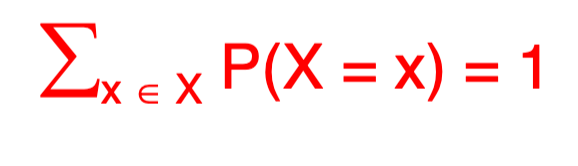
\includegraphics[width=\textwidth/4]{7.png}
    \item Continuous RV:
    \item 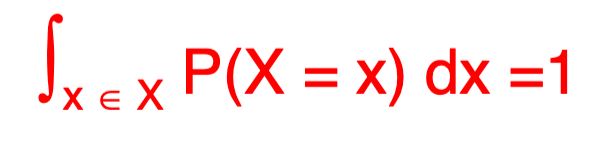
\includegraphics[width=\textwidth/4]{8.png}
  \end{itemize}
  \item Write P(x) for P(X=x), write P(X) for full distribution
  \item Representing probability distributions
  \begin{itemize}
    \item Discrete (finite) RV: tabular
    \item Continuous (infinite) RV: function
  \end{itemize}
\end{itemize}
\subsection{Joint Distributions on RVs}
Aliens in your backyard

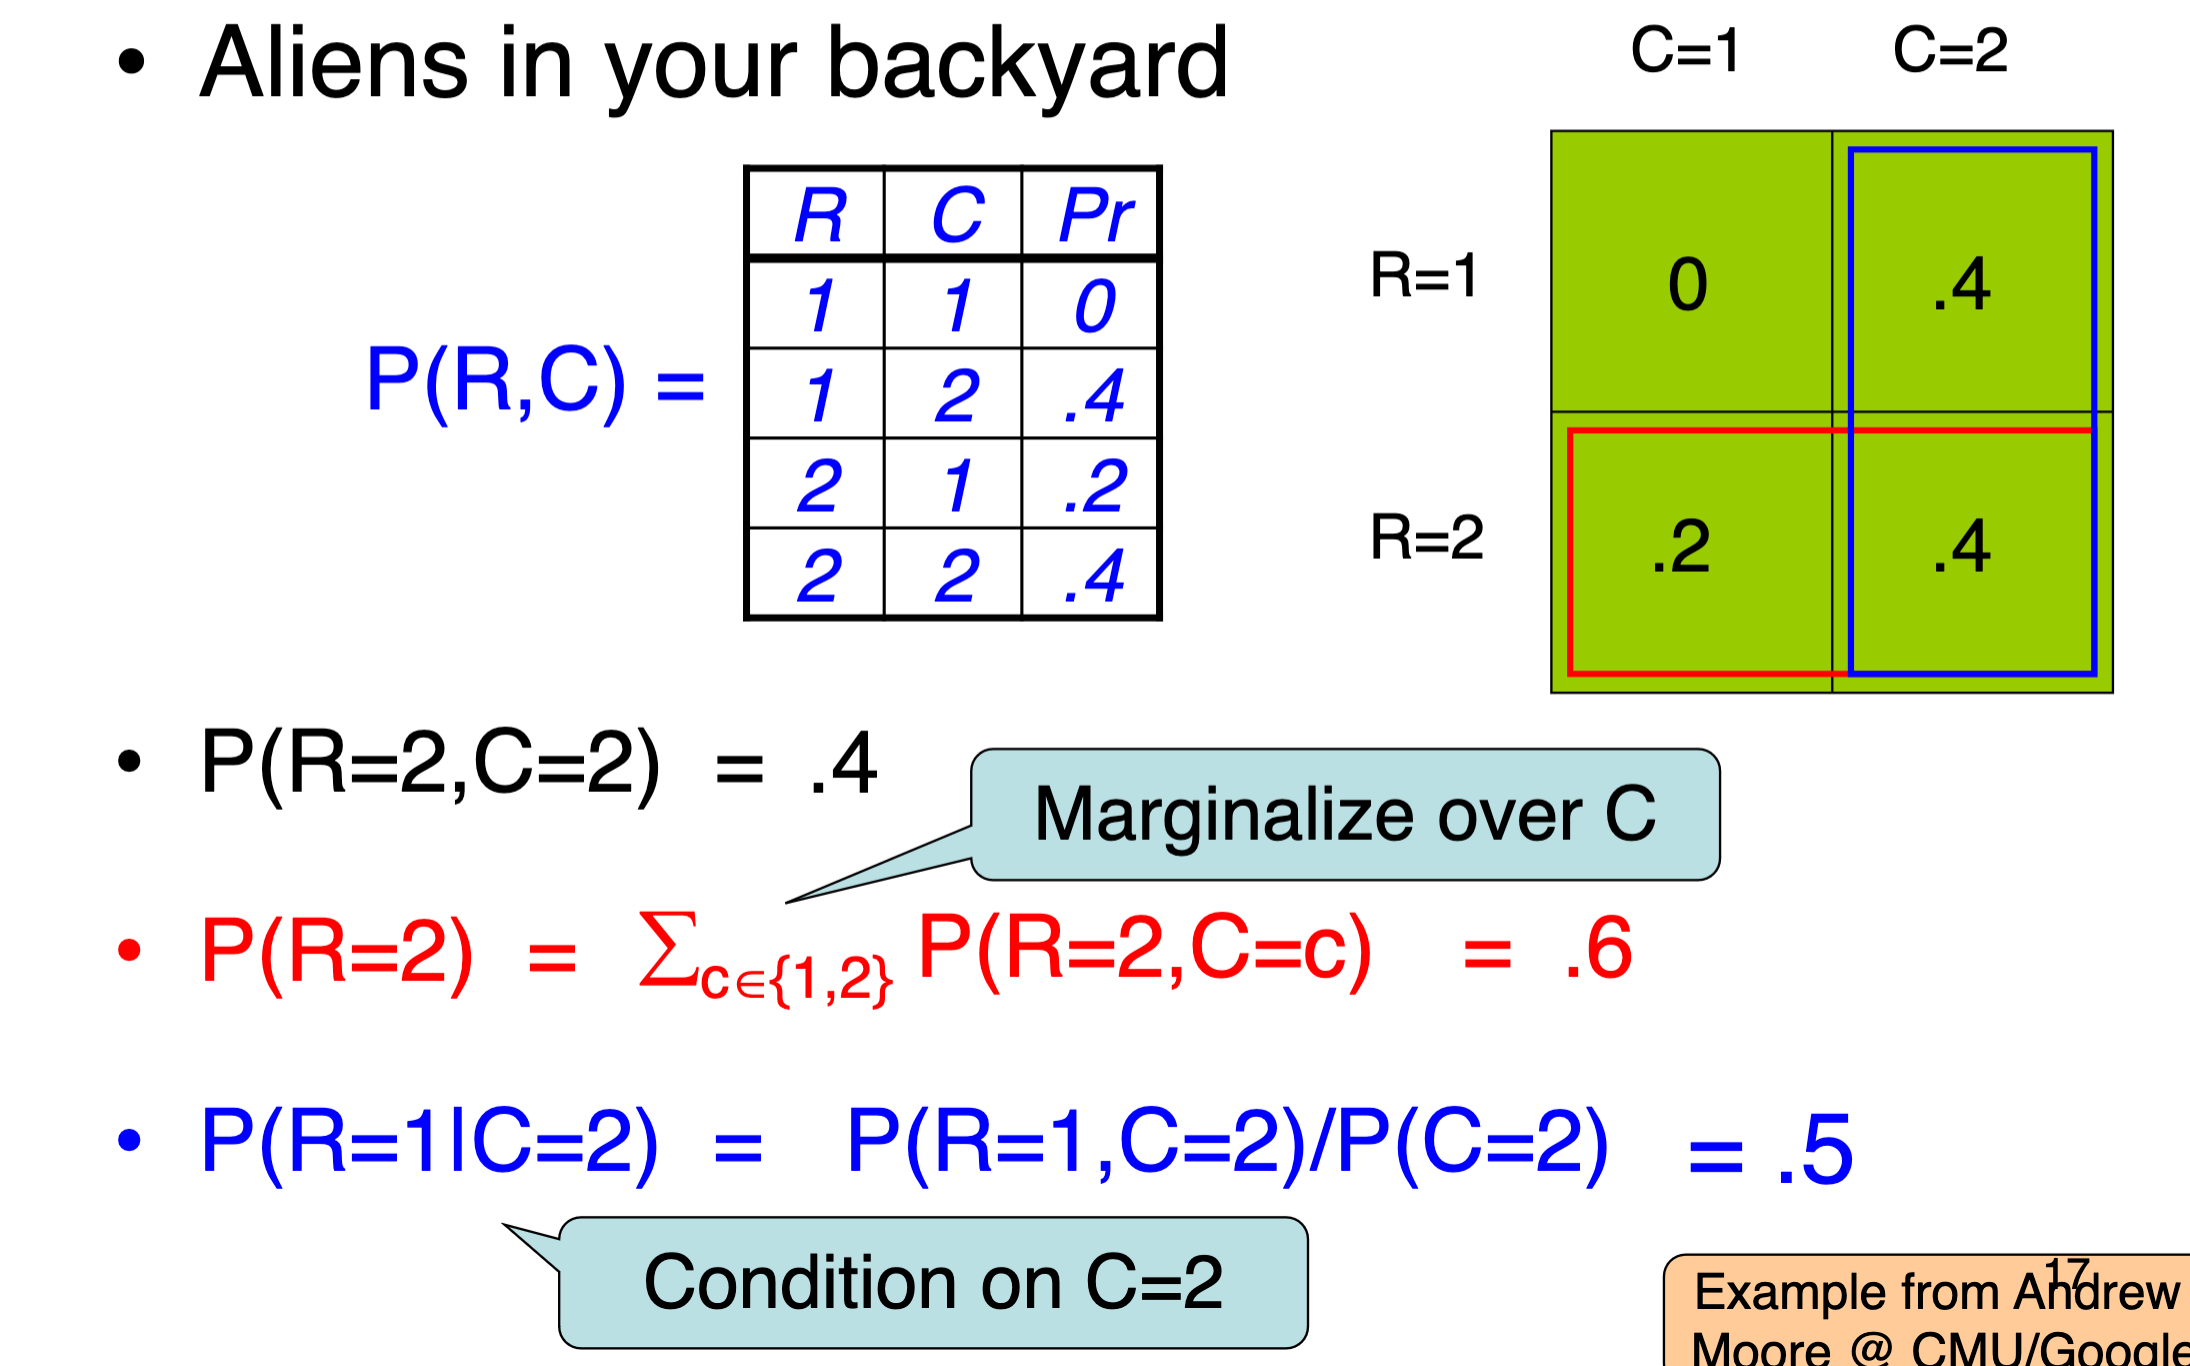
\includegraphics[width=\textwidth]{6.png}

\end{document}